\documentclass[9pt,a4paper,unknownkeysallowed,xcolor=dvipsnames,aspectratio=43]{beamer}
\usepackage{lastpage}
\usepackage{graphicx}
\usepackage{hyperref}  
\usepackage{bm,amsmath,amssymb}
\usepackage{slashed}

%\usepackage[dvipsnames]{xcolor}
\definecolor{darkred}{RGB}{212, 0, 0}
\definecolor{darkgreen}{RGB}{0,128,0}
\definecolor{teablue}{RGB}{67,0,181}
\definecolor{darkblue}{RGB}{0,0,128}
\hypersetup{
    colorlinks=true,
    linkcolor=blue,
    filecolor=magenta,      
    urlcolor=blue,
    citecolor=blue
}
\newcommand{\currentpage}{\thepage / \pageref{LastPage}}
\setbeamertemplate{footline}
{
  \leavevmode%
  \hbox{%
\footnotesize\sffamily
  \begin{beamercolorbox}[wd=.40\paperwidth,ht=3ex,dp=1ex,center]{}%
   \color{teablue} Jet Physics
  \end{beamercolorbox}%
  \begin{beamercolorbox}[wd=.20\paperwidth,ht=3ex,dp=1ex,center]{}%
  \currentpage 
  \end{beamercolorbox}%
  \begin{beamercolorbox}[wd=.40\paperwidth,ht=3ex,dp=1ex,center]{}%
   \color{teablue} 2. QCD and Jets
  \end{beamercolorbox}%
}
}
\setbeamertemplate{frametitle}[default][center]
\begin{document}


\begin{frame}
\topskip0pt
\vspace*{\fill}
\begin{center}
{\Huge\bf\color{darkred} Introduction to Jet Physics}\\
\vspace{4mm}
    Bin Wu\\
    \vspace{8mm}
    {\bf\Large Lecture 2: QCD and Jets}\\\vspace{4mm}
    {\color{darkblue} 15-04-2021}
\end{center}
\vspace{4mm}
\begin{itemize}
    \item[\color{darkred}\Large\bullet] Recap of QCD
    \vspace{2mm}
    \item[\color{darkred}\Large\bullet] Born dijet cross section
    \vspace{2mm}
    \item[\color{darkred}\Large\bullet] High-order jet cross section and factorization
    \vspace{2mm}
    \item[\color{darkred}\Large\bullet] Jets in perturbative QCD

\end{itemize}
\vspace*{\fill}
\end{frame}
%
%%%%%%%%%%%%%%%%%%%%%%%%%%%%%%%%%%%%%%%%%%%%%%%%%%%%%%%%%%
%
\begin{frame}{\bf\huge Recap of QCD}

{\color{darkred}\Large$\bullet$} {\color{darkred} The QCD Lagrangian}\\
\begin{align}
    \mathcal{L}=-\frac{1}{4}F^a_{\mu\nu}F^{a\mu\nu}+\sum\limits_f\bar{q}_f(iD_\mu\gamma^\mu-m_f)q_f
\end{align}
where $D_\mu=\partial_\mu-ig A_\mu$ and $F_{\mu\nu}=\partial_\mu A_\nu \partial_\nu A_\mu-ig[A_\mu,A_\nu]$ with $A_\mu\equiv A^a_\mu t^a$ and $t^a$ the $SU(N_C)$ generators in the fundamental representation. Here, $N_c = 3$ in the real world.
\vspace{2mm}

{\color{darkred}\Large$\bullet$} The color matrices obey\\
\begin{align}
    &[t^a, t^b] = i f^{abc} t^c,\qquad\text{Tr}[t^a t^b]=\frac{\delta^{ab}}{2},\notag\\
    &f^{abc}f^{abd}=C_A \delta^{cd},\qquad (t^a t^a)_{bc} = C_F \delta_{bc},
\end{align}
with $C_A\equiv N_c,\qquad C_F \equiv \frac{N_c^2 -1 }{2 N_c}$.
\end{frame}
%
%
%%%%%%%%%%%%%%%%%%%%%%%%%%%%%%%%%%%%%%%%%%%%%%%%%%%%%%%%%%
%
\begin{frame}

{\color{darkred}\Large$\bullet$} {The Feynman rules:}\\
\begin{center}
    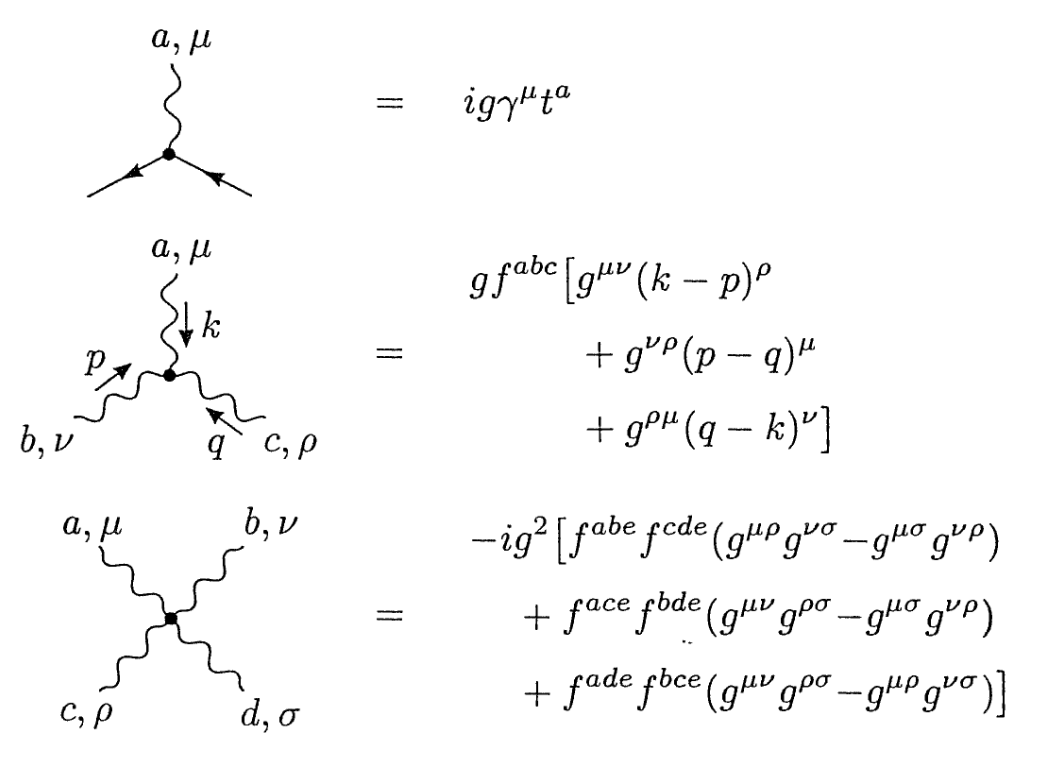
\includegraphics[width=0.7\textwidth]{02/FR.png}
\end{center}\\
quark propagator: $\frac{i(\slashed{p}+m_f)}{p^2 - m_f^2 + i\epsilon}$\\
gluon propagator in $\xi\cdot A = 0$ gauge: $\frac{-i}{p^2 + i\epsilon}\left(g^{\mu\nu}-\frac{\xi^\mu p^\nu + \xi^\nu p^\mu}{\xi\cdot p}\right)$
%When a non-physical gauge is used, there will be additional gauge-fixing terms from quantization.
\end{frame}
%
%%%%%%%%%%%%%%%%%%%%%%%%%%%%%%%%%%%%%%%%%%%%%%%%%%%%%%%%%%
%
\begin{frame}\vspace{2mm}

{\color{darkred}\Large$\bullet$} QCD is renormalizable and all ultraviolet (UV) divergences can be removed by redefining the coupling constant, quark masses and the field strengths. This renormalization procedure introduces some renormalization scale $\mu$.\\
\vspace{1mm}

{\color{darkred}\Large$\bullet$} {\color{darkred} The running coupling}: $\alpha_s(\mu)\equiv \frac{g^2(\mu)}{4\pi}$\\
\begin{align}
\frac{d\alpha_s(\mu)}{d\log\mu}=\beta(\alpha_s(\mu)),~~~\beta(\alpha_s) = -2\alpha_s \sum_{n=0}^{\infty}\beta_n \left( \frac{\alpha_s}{4\pi} \right)^{n+1}
\end{align}
with
\begin{align}
\beta_0\equiv \frac{11}{3}C_A-\frac{2}{3}n_f,\qquad\beta_1=\frac{34}{3} C_A^2-\frac{10}{3}C_A n_f-2 C_F n_f.
\end{align}

\begin{center}
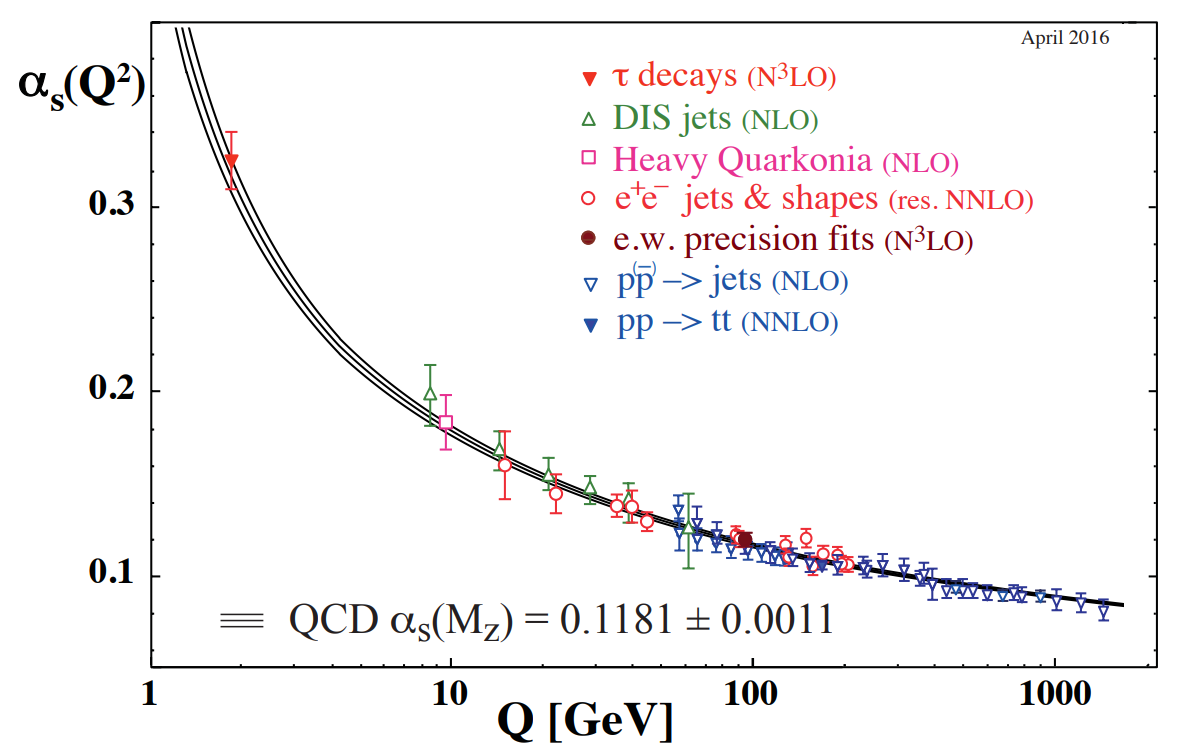
\includegraphics[width=0.5\textwidth]{02/alphas.png}\\
{\tiny \color{teablue}S.~Bethke,
  %\emph{{Pre-2019 summaries of $\alpha_s$}},
  \href{https://doi.org/10.22323/1.365.0001}{\emph{PoS} {\bfseries ALPHAS2019}
  (2019) 001}.}\\
\end{center}
\end{frame}
%
%%%%%%%%%%%%%%%%%%%%%%%%%%%%%%%%%%%%%%%%%%%%%%%%%%%%%%%%%%
%
\begin{frame}\vspace{2mm}

{\color{darkred}\Large$\bullet$} QCD shows {\color{darkred}asymptotic freedom} at short distance: $\alpha_s(Q\to 0)$ as $Q\to \infty$. Therefore, we can safely use pertrubation theory at large $Q$.
\vspace{2mm}

{\color{darkred}\Large$\bullet$} QCD becomes {\color{darkred}nonperturbative} at long distances, which is characterized by a low momentum scale: {\color{darkred} the Lambda parameter} defined as\\
\begin{align}
\log\frac{Q}{\Lambda}=-\int_{\alpha_s(Q)}^\infty\frac{d\alpha_s}{\beta(\alpha_s)}
\end{align}
That is, $\alpha_s(Q)\to \infty$ as $Q\to \Lambda$. At one loop, one has
\begin{align}
\log\frac{Q}{\Lambda} = \frac{2\pi}{\beta_0 \alpha_s(Q)}.    
\end{align}
$\Lambda\approx 200$ MeV $\approx$ 1/(proton size) sets the scale of {\color{darkred} nonperturbative physics} although its exact value depends on the renormalization scheme when $\beta$ is calculated up to high orders in $\alpha_s$.
\vspace{2mm}

{\color{darkred}\Large$\bullet$} A parton with $p^\mu$ can be described by perturbative QCD when {\color{darkred} its virtuality} $|p^2|\gg \Lambda^2$.
\vspace{2mm}
\end{frame}
%
%%%%%%%%%%%%%%%%%%%%%%%%%%%%%%%%%%%%%%%%%%%%%%%%%%%%%%%%%%
%
\begin{frame}\vspace{2mm}

{\color{darkred}\Large$\bullet$} Typical nonperturbative physics with $\sqrt{|p^2|}\sim \Lambda$ includes:
\vspace{2mm}
\begin{enumerate}
    \item[\diamondsuit] {\color{darkred}Confinement:} {\it that fact that quarks and gluons are found only in hadrons.}\\\vspace{2mm}
    It is a static properties of QCD, which can be studied from QCD first principles using lattice simulations.
    \vspace{2mm}
    \item[\diamondsuit] {\color{darkred}Hadronization:} {\it a dynamical process in which partons convert into hadrons.}\\\vspace{2mm}
    The quantitative description of hadronization has only been done by models. Heuristically, hadronization takes place within
    \begin{align}
        t_h\sim \left\{
        \begin{array}{ll}
             \frac{1}{p}\sim 1~\text{fm} & \text{in the rest frame} \\
             \frac{E}{p_\perp^2}\sim \frac{E}{\Lambda}~\text{fm} & \text{if the parton is energetic}
        \end{array}
        \right.\notag
    \end{align}
    Example: a quark with energy $E = 200$ GeV behaves as a colored particle within the hadronization time $t_h\sim 10^3$ fm.\\\vspace{2mm}
    \begin{center}
        {\tiny \color{teablue}Y.L.~Dokshitzer, V.A.~Khoze, A.H.~Mueller and S.I.~Troian, \href{https://www.lpthe.jussieu.fr/~yuri/BPQCD/BPQCD.pdf}{\emph{{Basics of
  perturbative QCD}} (1991)}.
  }
    \end{center}
\end{enumerate}
\end{frame}
%
%%%%%%%%%%%%%%%%%%%%%%%%%%%%%%%%%%%%%%%%%%%%%%%%%%%%%%%%%%
%
\begin{frame}\vspace{2mm}

{\color{darkred}\Large$\bullet$} The collimated parton shower is closely related to {\color{darkred} infrared (IR) (soft and collinear) singularities} in (massless) perturbation theory. 
\vspace{2mm}
\begin{center}
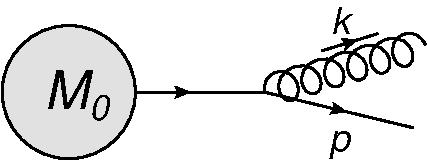
\includegraphics[width=0.3\textwidth]{02/branch.pdf}
\end{center}
$$
(p+k)^2=2 p\cdot k = 2 E_p E_k (1-\cos\Delta \phi)
$$
\begin{enumerate}
    \item {\color{darkred}Soft singularity:} $E_k\to 0$
    \item {\color{darkred}Collinear singularity:} $\Delta\phi\to 0$
\end{enumerate}
\vspace{2mm}

{\color{darkred}\Large$\bullet$} {\color{darkred}Infrared divergences show up even in hard processes} in hadron collisions, which indicate dependence on long-distance aspects of QCD.
\vspace{2mm}

{\color{darkred}\Large$\bullet$} Two classes of observable calculable using perturbation QCD:
\begin{enumerate}
    \item {\color{darkred}Infrared safe quantities:} infrared
divergences cancel between real and virtual contributions.
    \item {\color{darkred}Factorizable quantities:} infrared
divergences can be absorbed in universal nonperturbative objects, such as parton distribution functions (PDFs), fragmentation functions, etc.
\end{enumerate}

\end{frame}
%
%%%%%%%%%%%%%%%%%%%%%%%%%%%%%%%%%%%%%%%%%%%%%%%%%%%%%%%%%%
%
\begin{frame}{\bf\huge Born dijet cross section}
\vspace{2mm}

{\color{darkred}\Large$\bullet$} Recall the dijet event:
\begin{center}
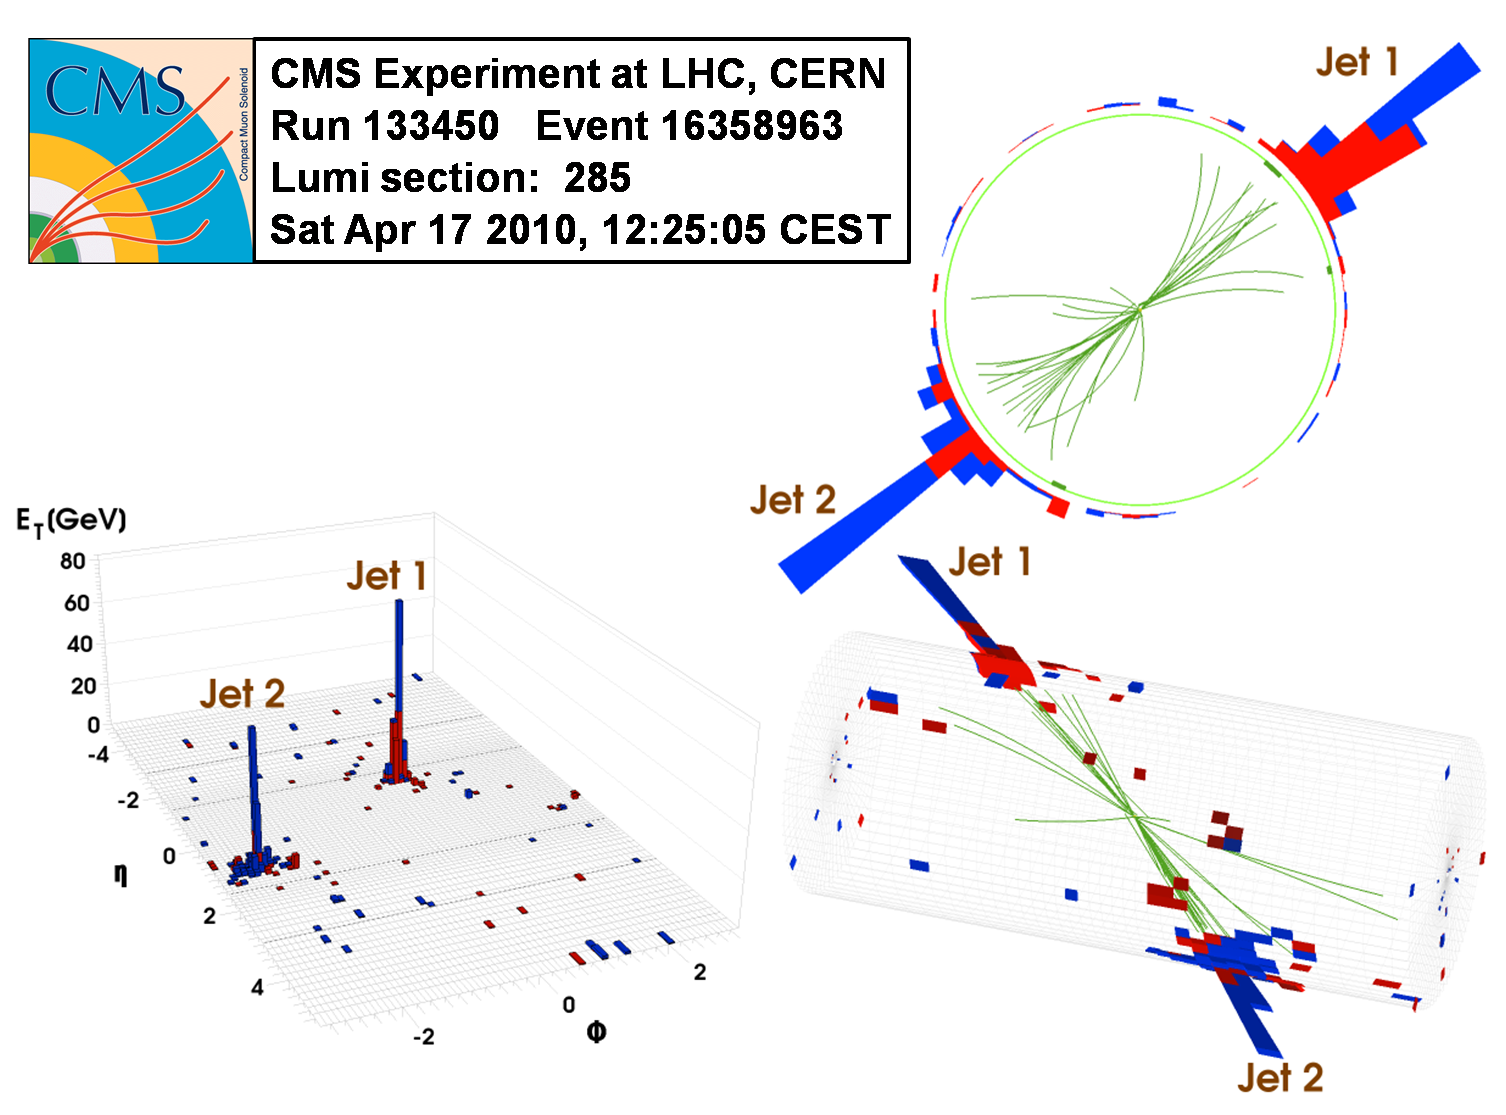
\includegraphics[width=0.8\textwidth]{01/lego.png}
\end{center}
\end{frame}
%
%%%%%%%%%%%%%%%%%%%%%%%%%%%%%%%%%%%%%%%%%%%%%%%%%%%%%%%%%%
%
\begin{frame}
\vspace{2mm}

{\color{darkred}\Large$\bullet$} Dijet cross section in pp collisions at tree level ($O(\alpha_s^2)$):
\begin{center}
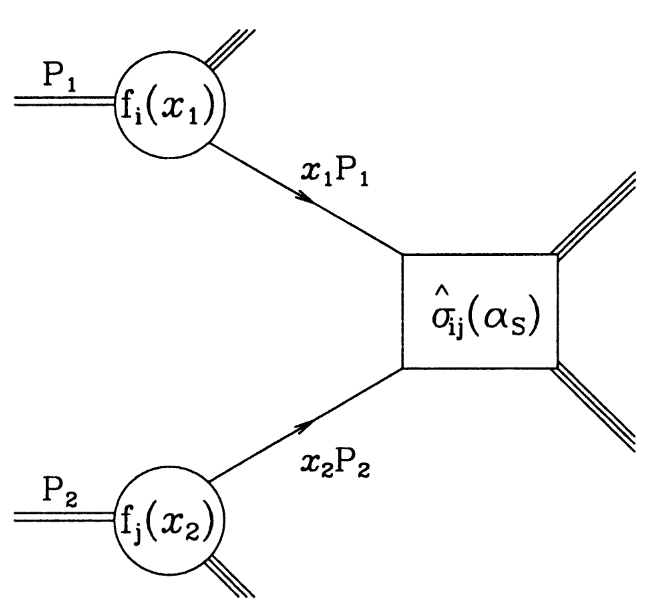
\includegraphics[width=0.5\textwidth]{02/dijetTree.png}
\end{center}
\begin{align}
    \frac{d\sigma}{dy_1 d^2p_{1T} dy_2 d^2p_{2T}} = \int dx_1 dx_2 f_i(x_1)f_j(x_2)\frac{d\hat{\sigma}_{ij}}{dy_1 d^2p_{1T} dy_2 d^2p_{2T}}
\end{align}
where $f_i, f_j$: PDFs, $\hat{\sigma}_{ij}$: partonic cross section.
\end{frame}
%
%%%%%%%%%%%%%%%%%%%%%%%%%%%%%%%%%%%%%%%%%%%%%%%%%%%%%%%%%%
%
\begin{frame}
\vspace{2mm}
\begin{columns}
\column{0.4\textwidth}
\begin{center}
    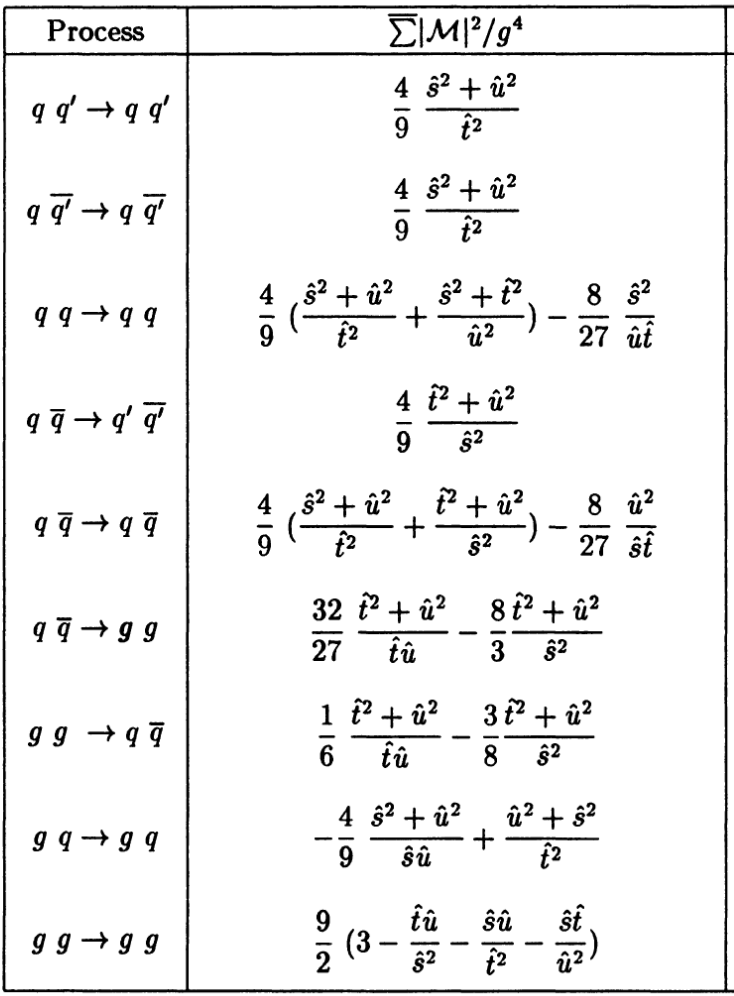
\includegraphics[width=\textwidth]{02/2to2.png}\\
    \vspace{1mm}
    {\tiny The color and spin indices are averaged (summed) over initial (final) states.}
\end{center}
\column{0.5\textwidth}
\begin{enumerate}
    \item<1-> Partonic di-jet cross section:
    \begin{align}
        &\frac{d\hat{\sigma}_{ij}}{dy_1 d^2p_{1T} dy_2 d^2p_{2T}}=\frac{1}{32\pi^2 x_1 x_2 s}\\
        &\times \overline{\sum} |\mathcal{M}|^2\delta^{(4)}(x_1P_1+x_2 P_2 - p_1 -p_2)\notag
    \end{align}
    with $s=(P_1 + P_2)^2$.
    \item<2-> Dijet cross section:
    \begin{align}\label{eq:sigdijet}
        &\frac{d\sigma}{dy_1 d^2p_{1T} dy_2 d^2p_{2T}}=\frac{1}{16\pi^2 s^2}\frac{f_i(x_1)}{x_1}\frac{f_j(x_2)}{x_2}\notag\\
        &\times \overline{\sum} |\mathcal{M}|^2\delta^{(2)}(\vec{p}_{1T} + \vec{p}_{2T})
    \end{align}
    with additional symmetric factor for final-state identical particles. 
\end{enumerate}
\end{columns}
\begin{center}
    {\color{darkred} HW2: Derive Eq. (\ref{eq:sigdijet}) and find out the expressions for $x_1$ and $x_2$.}
\end{center}
\end{frame}
%
%%%%%%%%%%%%%%%%%%%%%%%%%%%%%%%%%%%%%%%%%%%%%%%%%%%%%%%%%%
%
\begin{frame}{\bf\huge High-order jet cross section and factorization}
\vspace{2mm}

{\color{darkred}\Large$\bullet$} At high order in $\alpha_s$, one could encounter
\vspace{2mm}
\begin{itemize}
    \item[\diamondsuit] {\color{darkred}UV divergences} are removed by renormalization
    \vspace{2mm}
    \item[\diamondsuit] {\color{darkred} IR divergences} (in the massless limit)
    \vspace{2mm}
    \begin{enumerate}
        \item {from radiation collinear to beam directions {\color{darkred}DO NOT} cancel } $\Rightarrow$ PDFs
        \vspace{2mm}
        \item {from radiation collinear to jet directions cancel} by choosing jet definition
        \vspace{2mm}
        \item {from soft radiation cancel}. (This is, however, the most tricky part to prove factorization).
    \end{enumerate}
    \vspace{2mm}
    These are the main ingredients for the factorization formula.
        \vspace{2mm}
    % \item[\diamondsuit] {\color{darkred} Large logarithms}: resummation up to all orders in $\alpha_s$
    % \begin{align}
    %     \sigma \sim \exp\{\underbrace{g_1\alpha_s L^2}_{\text{LL}} + \underbrace{g_2\alpha_s L}_{\text{NLL}}+\underbrace{g_3\alpha_s^2 L}_{\text{NNLL}}+\cdots\}\notag
    % \end{align}
\end{itemize}

{\color{darkred}\Large$\bullet$} {\color{darkred}Contributions from collinear (and soft) radiation factorize}. To discuss the main features of the factorization formula, it is enough to focus on radiation which is both collinear and soft.\\
\vspace{2mm}
%\begin{center}
    {\tiny For more rigorous approaches to collinear factorization, see reviews in perturbative QCD:\\\vspace{2mm} {\color{teablue}G.~Sterman, %\emph{{QCD at Short Distances: Jets and Factorization}},
  \href{https://doi.org/10.5506/APhysPolB.45.2205}{\emph{Acta Phys. Polon. B}
  {\bfseries 45} (2014) 2205}
  [\href{https://arxiv.org/abs/1412.5698}{{\ttfamily 1412.5698}}].}
 \vspace{2mm}
 
or in soft-collinear effective theory (SCET):\\\vspace{2mm}
    {\color{teablue}T.~Becher, A.~Broggio and A.~Ferroglia, %\emph{{Introduction to Soft-Collinear Effective Theory}},
    vol.~896, Springer (2015),
%  \href{https://doi.org/10.1007/978-3-319-14848-9}{10.1007/978-3-319-14848-9},
  [\href{https://arxiv.org/abs/1410.1892}{{\ttfamily 1410.1892}}].}

.}
%\end{center}
\vspace{2mm}
\end{frame}
%
%%%%%%%%%%%%%%%%%%%%%%%%%%%%%%%%%%%%%%%%%%%%%%%%%%%%%%%%%%
%
\begin{frame}
\vspace{2mm}

{\color{darkred}\Large$\bullet$} Assuming k is soft and colliner to $p_i$, one has
\begin{align}
    \sigma_{m+1}(p_1, p_2, \cdots, p_l, \cdots, p_m, k)= \frac{4 g^2 C_l}{|k_{\perp_l}|^2} \sigma_{m}(p_1, p_2, \cdots, p_l + k, \cdots, p_m)
\end{align}
where $C_l=C_A$ or $C_F$ if $l$ is a gluon or quark/antiquark respectively, $k_{\perp_l}$ is the transverse momentum with respect to the direction of the momentum of parton $l$.\\\vspace{2mm}
{\color{darkred}\Large$\bullet$} The sketch of the proof:
using $\bar{n}_i\cdot A=0$ gauge
\begin{align}
    \sum\limits_{\lambda} \epsilon_\lambda^\mu(k)\epsilon_\lambda^{*\nu}(k) = -g^{\mu\nu} + \frac{\bar{n}_i^\mu k^\nu + \bar{n}_i^\nu k^\mu}{\bar{n}_i\cdot k}\qquad\text{with $\bar{n}_i^\mu = (1, -\vec{\hat{p}}_i)$},
\end{align}
one can see that the leading contribution comes only from 
\begin{center}
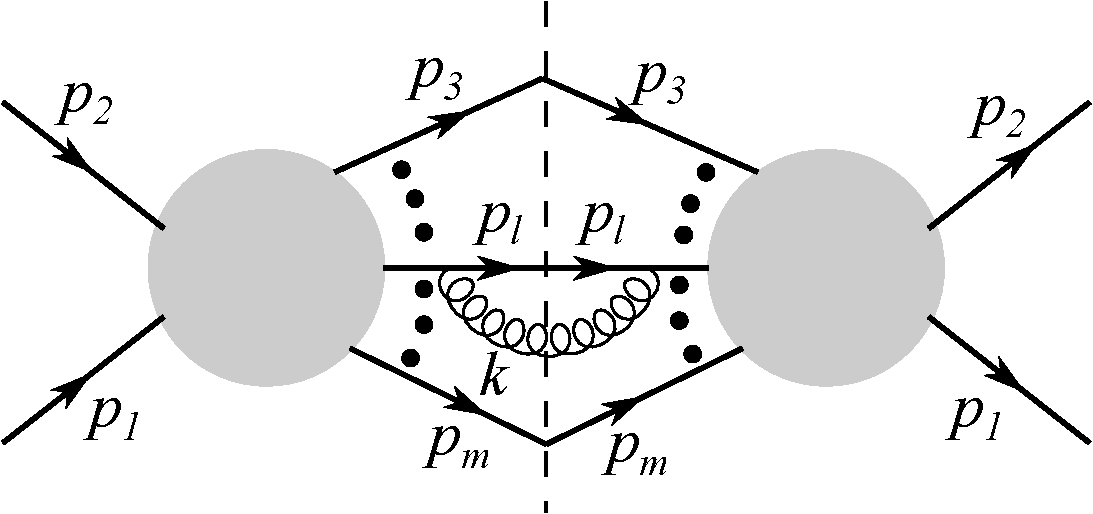
\includegraphics[width=0.5\textwidth]{02/main.pdf}
\end{center}


\end{frame}

%
%%%%%%%%%%%%%%%%%%%%%%%%%%%%%%%%%%%%%%%%%%%%%%%%%%%%%%%%%%
%
\begin{frame}
\vspace{2mm}

{\color{darkred}\Large$\bullet$} {\color{darkred}Contributions from emission of one soft real gluon:}
\begin{align}
    \left.\hat{\sigma}_{ij}\right|_{O(\alpha_s^3)} = \sum\limts_l \frac{\alpha_s C_l}{\pi^2}\int\frac{dz_l}{z_l}\int\frac{d^2 k_{\perp_ l}}{|k_{\perp_l}|^2}\left.\hat{\sigma}_{ij}\right|_{O(\alpha_s^2)}
\end{align}
where $l$ represents any of the two incoming and two outgoing partons at $O(\alpha_s^2)$.
\vspace{2mm}

{\color{darkred}\Large$\bullet$} If one only intends to get {\color{darkred}leading logarithmic (LL)} result, one can extend the limits of the integration in the above equation to the whole phase space, i.e.,
\begin{align}
    \left.\hat{\sigma}_{ij}\right|_{O(\alpha_s^3)} = \sum\limts_l \frac{2\alpha_s C_l}{\pi}\int_0^1\frac{dz_l}{z_l}\int_0^{Q}\frac{d k_{\perp_ l}}{k_{\perp_l}}\left.\hat{\sigma}_{ij}\right|_{O(\alpha_s^2)}
\end{align}

{\color{darkred}\Large$\bullet$} Similarly, at LL {\color{darkred}virtual diagrams in soft limit} give
\begin{align}
    \left.\hat{\sigma}_{ij}\right|_{O(\alpha_s^3)} = \sum\limts_l \left(-\frac{2\alpha_s C_l}{\pi}\right)\int_0^1\frac{dz_l}{z_l}\int_0^{Q}\frac{d k_{\perp_ l}}{k_{\perp_l}}\left.\hat{\sigma}_{ij}\right|_{O(\alpha_s^2)}
\end{align}

{\color{darkred}\Large$\bullet$} Both integrals are divergent but they cancel with each other for infrared safe quantities.

\end{frame}
%
%%%%%%%%%%%%%%%%%%%%%%%%%%%%%%%%%%%%%%%%%%%%%%%%%%%%%%%%%%
%
\begin{frame}
\vspace{2mm}

{\color{darkred}\Large$\bullet$} Corrections from (soft) radiation collinear to $P_1$:
\begin{align}
    \Delta \sigma_1= &\int dx_1' dx_2 f_i(x_1') f_j(x_2)\frac{2\alpha_s C_F}{\pi}\int_0^1\frac{dz}{z} \int_0^Q\frac{d k_T}{k_T}\notag\\
    &\times\int_0^1 d x_1 [\delta(x_1 - (1-z)x') - \delta(x_1-x_1')]\hat{\sigma}_{ij}
\end{align}
Then, by integrating out $x_1'$ and
% get
% \begin{align}
%     \Delta \sigma_1= &\int dx_1 dx_2  f_j(x_2)\frac{2\alpha_s C_F}{\pi}\int_0^1\frac{dz}{z} \int_0^Q\frac{d k_T}{k_T}\notag\\
%     &\times \left[\frac{1}{1-z} f_i\left(\frac{x_1}{1-z}\right) - f(x_1)\right]\hat{\sigma}_{ij}.
% \end{align}
% By 
changing the variable $z\to 1-z$, one has
\begin{align}
    \Delta \sigma_1= &\int dx_1 \frac{2\alpha_s C_F}{\pi}\int_{x_1}^1\frac{dz}{z} \int_0^Q\frac{d k_T}{k_T}\notag\\
    &\times \left[\frac{1}{1-z} f_i\left(\frac{x_1}{1-z}\right) - f_i(x_1)\right]\int dx_2  f_j(x_2)\hat{\sigma}_{ij}\notag\\    &\equiv \int dx_1 \frac{\alpha_s }{\pi}\int_0^Q\frac{d k_T}{k_T}\int_{x_1}^1\frac{dz}{z}P_{q\leftarrow q} f_i(\frac{x_1}{z})\int dx_2  f_j(x_2)\hat{\sigma}_{ij}.
\end{align}
We can see that
\begin{enumerate}
    \item {soft divergence cancels out;}
    \item at nonvanishing $z$, {there is collinear divergence.}
\end{enumerate}
{\color{darkred}The cross section for hard processes in hadron collisons is not infrared safe!}
\end{frame}
%
%%%%%%%%%%%%%%%%%%%%%%%%%%%%%%%%%%%%%%%%%%%%%%%%%%%%%%%%%%
%
\begin{frame}
\vspace{4mm}

{\color{darkred}\Large$\bullet$} Here, we encounter collinear divergence because we take the gluon as a massless onshell particle. However, we can not trust our perturbative calculation in the limit $k_T\to 0$.\\
\vspace{4mm}

{\color{darkred}\Large$\bullet$} We may put a lower cutoff $\Lambda$ to $k_T$-integral based on physical intuition and interpret $f_i$ as the PDF at scale $\Lambda$. That is, gluons in the proton typically has a transverse momentum of $O(\Lambda)$. \\
\vspace{4mm}

{\color{darkred}\Large$\bullet$} Equivalently, one may choose an arbitrary scale $\mu_F$ instead, which is called {\color{darkred}factorization scale}. In this case, the PDF depends on $\mu_F$ as well.\\
\vspace{4mm}
 
 {\color{darkred}\Large$\bullet$} Since $\mu_F$ is arbitrary, one should have
 \begin{align}
     \frac{d\Delta \sigma_1}{d\log \mu_F} =0 \Rightarrow \frac{d }{d\log \mu_F} f_{i}(x_1,\mu_F) = \frac{\alpha_s }{\pi}\int_{x_1}^1\frac{dz}{z}P_{q\leftarrow q} f_i(\frac{x_1}{z}, \mu_F)
 \end{align}
 which is {\color{darkred}the DGLAP equation} in soft limit ($z\to 1$).\\\vspace{4mm}
 
 {\color{darkred}\Large$\bullet$} The argument above is obviously valid for $f_j$ and for all other hard processes. Therefore, PDFs are {\color{darkred}universal}, which can be measured experimentally. 
\end{frame}
%
%%%%%%%%%%%%%%%%%%%%%%%%%%%%%%%%%%%%%%%%%%%%%%%%%%%%%%%%%%
%
\begin{frame}

{\color{darkred}\Large$\bullet$} Additional IR singularities could arise from radiation collinear to jet directions since both real and virtual diagrams contain IR singularities.\\\vspace{2mm}

{\color{darkred}\Large$\bullet$} To obtain a finite cross section, {\color{darkred}jets are hence required to be infrared (soft) and collinear (IRC) safe}, which, for an observable $V$, means
\begin{align}
\text{collinear safety:}&&
V_{m+1}\left(\ldots,k_i,k_j,\ldots\right)&\longrightarrow V_{m}\left(\ldots,k_i+k_j,\ldots\right) &&\mathrm{if}\;k_i\parallel k_j ,\notag\\
\text{infrared safety:}&&
V_{m+1}\left(\ldots,k_i,\ldots\right)&\longrightarrow V_{m}\left(\ldots,k_{i-1},k_{i+1},\ldots\right) &&\mathrm{if}\;k_i\to 0.\notag
\end{align}

{\color{darkred}\Large$\bullet$} {\color{darkred}The factorization formula} at leading order in $Q$ (leading twist)
\begin{equation}
\sigma = \int_0^1 dx_1 dx_2 \int d\Phi_n f_i^{h_1}(x_1,\mu_F) f_j^{h_2}(x_2, \mu_F) \frac{1}{2 \hat{s}} |\mathcal{M}_{ij \to n}|^2(\Phi_n;\mu_F,\mu_R)\;,
\label{eq:master}
\end{equation}
where $\mu_F$ is the factorisation scale and
\begin{equation}
d\Phi_n = \left[\prod_{a=1}^{n} \frac{d^3p_a}{(2\pi)^3 2 E_a} \right](2 \pi)^4 \delta^{(4)}(p_i + p_j - \sum_{a=1}^{n} p_a)\;.
\label{eq:dLIPS}
\end{equation}

{
The IR safety of jets ensures that the cross section does not contain any IR singularities and perturative QCD is valid. 
}
\end{frame}
%
%%%%%%%%%%%%%%%%%%%%%%%%%%%%%%%%%%%%%%%%%%%%%%%%%%%%%%%%%%
%
\begin{frame}
\vspace{2mm}

{\color{darkred}\Large$\bullet$} {\color{darkred} Fixed-order calcuation based on factorization formula:} inclusive jet cross section at NLO:
\begin{center}
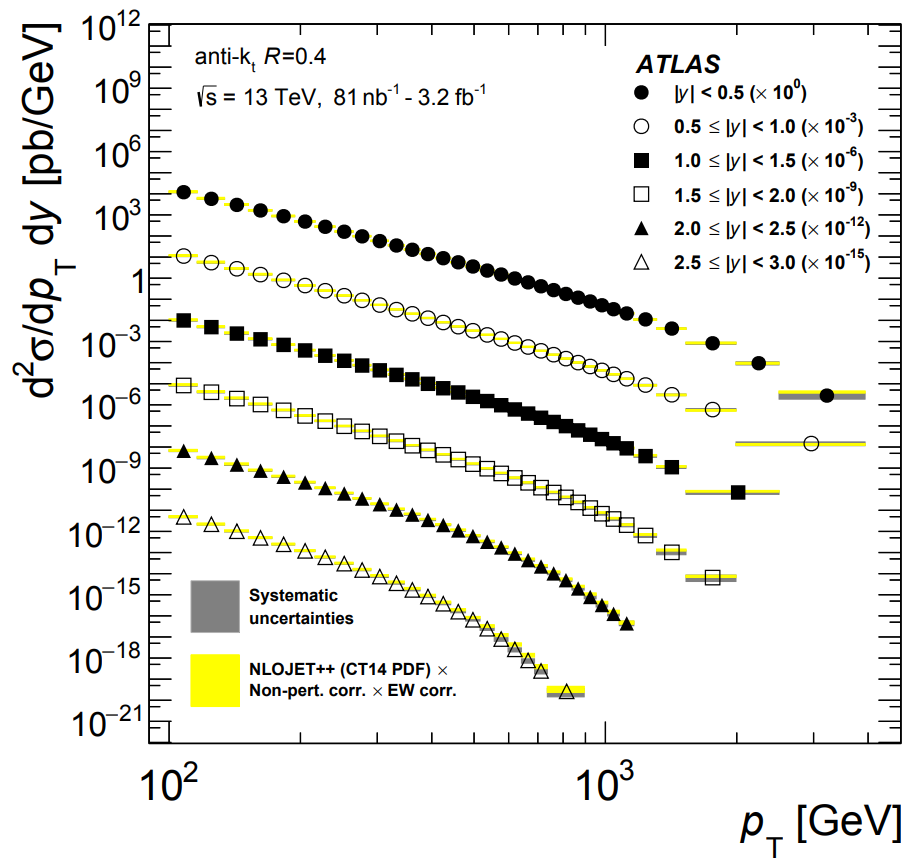
\includegraphics[width=0.6\textwidth]{02/inclusivejet.png}\\\vspace{1mm}
NLO pQCD predictions and the CT14 NLO PDF set\\\vspace{1mm}
{\tiny \color{teablue} {\scshape ATLAS} collaboration, %\emph{{Measurement of inclusive jet and dijet cross-sections in proton-proton collisions at $\sqrt{s}=13$ TeV with the ATLAS detector}},
  \href{https://doi.org/10.1007/JHEP05(2018)195}{\emph{JHEP}
  {\bfseries 05} (2018) 195}
  [\href{https://arxiv.org/abs/1711.02692}{{\ttfamily 1711.02692}}].}
\end{center}
\end{frame}
%
%%%%%%%%%%%%%%%%%%%%%%%%%%%%%%%%%%%%%%%%%%%%%%%%%%%%%%%%%%
%
\begin{frame}{\bf\huge Jets in perturbative QCD}
\vspace{2mm}

{\color{darkred}\Large$\bullet$} Jets connect short-distance physics to long-distance physics:
\vspace{2mm}
\begin{align}
\sigma_{jet}=\begin{array}{c}
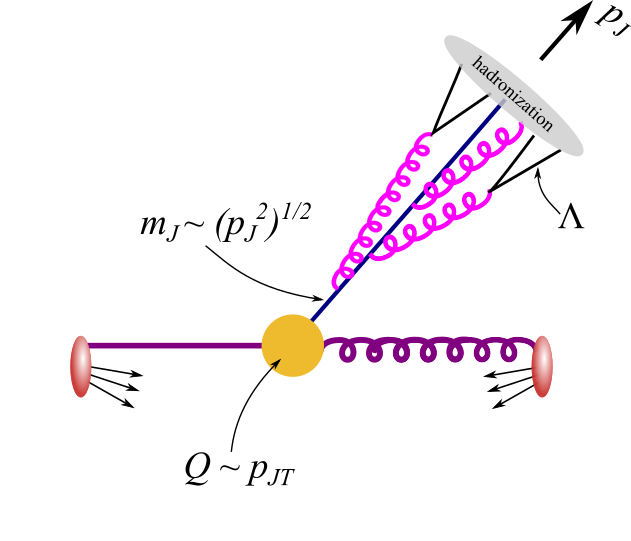
\includegraphics[width=0.5\textwidth]{02/jetpQCD.png}
\end{array}
\end{align}
There are three scales: $p_{JT} \gg m_J \gg \Lambda$.

\end{frame}
%
%%%%%%%%%%%%%%%%%%%%%%%%%%%%%%%%%%%%%%%%%%%%%%%%%%%%%%%%%%
%
\begin{frame}{\bf\huge Jets in perturbative QCD}
\vspace{2mm}

{\color{darkred}\Large$\bullet$} IRC safety $\Rightarrow$ nonperturbative effects of $O(\Lambda/p_{JT})$:
\vspace{2mm}
\begin{align}
\sigma_{jet}=\begin{array}{c}
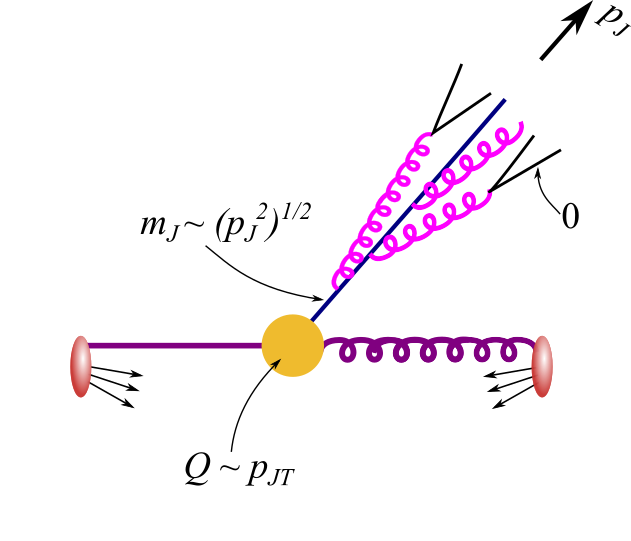
\includegraphics[width=0.5\textwidth]{02/jetparton.png}
\end{array} + O(\Lambda/p_{JT})
\end{align}
The requirement of IRC safety means that an observable can be computed reliably in perturbative QCD,
up to non-perturbative power corrections, which decrease as the hard scale of the process increases.
\end{frame}

\end{document}